

\section{Unstrukturierter Text versus strukturierte Daten?}


\begin{frame}{Text als unstrukturierte Daten?}
\begin{enumerate}
    \item Tabellendaten $\to$ strukturierte Daten $\to$ Information Retrieval
    \item Text $\to$ notorisch unstrukturierte Daten
    \item Wie kann man
    \begin{enumerate}
        \item Text digital modellieren/abbilden?
        \item Text abfragbar machen (Textmining)
    \end{enumerate}
    \item Data Mining / Data Science versus Textmining?
\end{enumerate}
    
\end{frame}
%------------------------------------------------------------------------------

\begin{frame}{Text versus Tabellendaten}

\red{Im Gegensatz zum \emph{Information Retrieval} aus DBs}
Relevante Strukturen erst identifizieren, nicht Informationen, von denen man schon weiß, dass sie drin sind, lediglich extrahieren. 
\bigskip

\metroset{block=fill}
\begin{block}{}
\begin{quote}\footnotesize
    \punkti you \emph{reduce} a text to a few elements, and \emph{abstract} them from the narrative flow, and construct a new, \emph{artificial} object. \punkti And with a little luck, these maps will \punkti possess `emerging' qualities, which were not visible at the lower level. \punkti Not that the map itself is an explanation, of course. It offers a model \punkti\footcite[53]{graphsmoretti} 
\end{quote}
\end{block}
\end{frame}
%------------------------------------------------------------------------------

\begin{frame}[allowframebreaks]{Quantitative Textanalyse}
\metroset{block=fill}

\begin{block}{}
\begin{quote}
    Reading `more' seems hardly to be the solution. Especially because we've just started rediscovering what Margaret Cohen calls the `great unread'. \lbrack{} Apart from ``its canonical fraction, which is not even 1 per cent of published literature''\rbrack{} there are \lbrack{}thousands of books\rbrack{} -- no one really knows, no one has read them, no one ever will.\footcite[45]{distantreading} 
\end{quote}
\end{block}

\red{Franco Morettis \emph{Distant Reading}} 
\begin{itemize}\footnotesize
    \item Vorstellung serielles Lesen vs. menschliches \emph{Close Reading}. 
    \item Behauptet, Literaturwissenschaft wäre nicht mehr vollständig ohne quantitative Aspekte. Das serielle Lesen aber auch irgendwie `als Alternative' anstatt \emph{close reading}.
\end{itemize}

\framebreak

\green{Matthew Jockers's \emph{Macroanalysis}}
Vorstellung einer Zoom-Bewegung: Die quantitative Analyse bietet Anstöße für das \emph{Close Reading}, etc.
Er fordert die Unterscheidung zwischen \emph{reading} und \emph{analysis} -- der Überblick `aus der Ferne' ist für ihn nicht `Lesen', wie etwa Morettis Benennung suggerieren würde.

\begin{enumerate}\footnotesize
    \item Kontextualisierung durch das \emph{zooming out}
    \item andererseits aber auch extremes \emph{close reading}: So viel Details wie dem Computer können einem Menschen fast gar nicht auffallen, weil wir Details ja gar nicht so richtig wahrnehmen.
    \item besser informiertes Verstehen der Primärtexte: die \emph{macroscale} gibt weniger `anekdotische' Beweise als das sehr genaue Lesen nur eines einzigen Texts.
    \item `harvesting findings, not facts'
    %\item `Mixed Methods'-Ansatz, Wechselspiel
\end{enumerate}

\begin{block}{}
\begin{quote}
    This is not close reading; this is macroanalysis, and the strength of the approach is that it allows for both zooming in and zooming out.\footcite[23]{macroanalysis}
\end{quote}
\end{block}
%\red{Pipers \emph{cultural analytics}}

\end{frame}
%------------------------------------------------------------------------------

\begin{frame}{Unterschiedliche Namen für dieselbe Sache?}
\metroset{block=fill}
\begin{block}{NLP}
Natural Language Processing, Computer-Sprachverarbeitung (Text und Audio) im Allgemeinen, bedient sich der \emph{Computerlinguistik}.
\end{block}

\begin{block}{Text Mining}
\begin{quote}
    Text mining, also referred to as text data mining, roughly equivalent to text analytics, is the process of deriving high-quality information from text. High-quality information is typically derived through the devising of patterns and trends through means such as statistical pattern learning. (\href{https://en.wikipedia.org/wiki/Text_mining}{Wikipedia})
\end{quote}
\end{block}

\begin{block}{Distant Reading}\footnotesize
Der Begriff bezeichnet in den Geisteswissenschaften quantitative Textanalyse (sonst ist es eher \emph{text mining}). Popularisiert durch Franco Moretti steht er als Gegensatz zur typisch geisteswissenschaftlichen Methode des \emph{close reading} aus der Literaturwissenschaft. \emph{Distant Reading} ist daher eher im Bereich der Computerphilologie (CLS, Computational Literary Studies) anzusiedeln.
\end{block}
\end{frame}
%------------------------------------------------------------------------------


%------------------------------------------------------------------------------


\begin{frame}{Natural Language Processing (NLP)}
\subsection{Natural Language Processing (NLP)}

\begin{columns}
\column{0.55\textwidth}
\begin{itemize}
\item \alert{Achtung Verwechslungsgefahr!} NLP = \emph{Natural Language Processing} $\neq$ \emph{Neurolinguistic Programming}
\item heute omnipräsent: 
\begin{itemize}\footnotesize
\item Sprachassistenten
\item maschinelle Übersetzung
\item wichtiges Element in \emph{Artificial Intelligence} $\to$ \emph{Turing Test} als Erfolgsmaß: Kann ein Computer vorgaukeln, ein Mensch zu sein? Dazu ist Sprache extrem wichtig.
\item Auto-Correct, Auto-Complete, \dots
\item Suchanfragen, \dots
\end{itemize}
\end{itemize}

\column{0.35\textwidth}
\metroset{block=fill}\scriptsize
\begin{block}{NLP-Tools}
Für `lebendige' Sprachen gibt es mittlerweile eigentlich von fast jeder Programmiersprache etwas.
\begin{description}
\item[Python] NLTK (Natural Language Toolkit), CLTK (Classical Language Toolkit)
\item[R] Stylo, tm, tidyr
\item[Java] CoreNLP, Mallet, \dots
\end{description}
\end{block}

\end{columns}

\end{frame}
%------------------------------------------------------------------------------




\begin{frame}[allowframebreaks]{Automatisierte Sprachverarbeitung mit Natural Language Processing-Pipeline}

Bevor wir mit der Verarbeitung beginnen können, ist 
\alert{(\emph{Pre-Processing})} 
nötig, weil ja Text eine `messy', also chaotische, unsaubere, unstrukturierte Datenform ist. Wir müssen die Strukturen darin erst für Computer `mundgerecht' verarbeiten und explizit machen.

Erster Schritt ist dabei die \alert{Tokenisierung} = d.h. Worterkennung / Aufspaltung eines Texts in Einzelwörter.

\metroset{block=fill}
\begin{block}{}\footnotesize
\begin{quote}
    \textbf{But what is a word?} We tend to think of a word as a unit of meaning that often has an analog in the real world. \punkti A computer doesn't know what a word is and certainly has no sense of what words might refer to.
    \punkti 
    Words are usually bounded by spaces and punctuation, and a computer can be told to split a long string (text) into shorter strings (words) by looking for the demarcation characters \punkti -- a process called tokenization.\footcite[283]{textvisual}
\end{quote}
\end{block}

\smallskip

\red{Tokenizer}
\begin{itemize}\footnotesize
    \item \textbf{Einfachste Tokenizer:} Nur der Whitespace/Leerzeichen ist Trenner. Erweiterbar durch Hinzufügen von Punktuation oder sprachinternen Spezifika.
    \item \textbf{Sprachgebunden}, z.B. frz. \emph{l'enfant}, lat. \emph{dixitque}, en. \emph{don't} auflösen, \dots 
    \item Wie wird mit \textbf{\emph{compounds}} (zusammengesetzen Wörtern) umgegangen? Fremdsprachliche \textbf{Lehnwörter}, die zusätzlich noch stehende Wendungen sind (z.B. \emph{en masse})?
    \item Geht meist ohne Wörterbuch -- für die meisten anderen NLP-Methoden müssen Wörterbücher und Grammatiken vorliegen (!) $\to$ für historischen Sprachstatus nicht selbstverständlich vorhanden.
\end{itemize}


\framebreak

\red{Lemmatization} Mithilfe von \textbf{Wörterbuch/Vokabular, Grammatik und morphologischer Analyse} der Wörter die Grundform (das \emph{Lemma}, wie man es im Wörterbuch hat) zu finden, damit alle Wortformen korrekt als Formen desselben \emph{type} gezählt werden können.

\bigskip

\red{Stemming} Wortende bis zur Wurzel abschneiden, nicht unbedingt auf linguistisch korrekte Art und Weise.

Weiterhin \red{Parsing, POS tagging, \emph{Named Entity Recognition} (NER), \dots}


\end{frame}
%------------------------------------------------------------------------------




\begin{frame}{Worthäufigkeitszählung (Quantitative Textanalyse)}
\begin{columns}
\column{0.5\textwidth}
Tokenisierung von Text; Auszählung der Worthäufigkeiten in einem 
\red{Bag-of-words (BOW)}
\green{\emph{type} vs. \emph{token}}
\smallskip

\emph{To be or not to be.} \\ = 6 \emph{tokens}, 4 \emph{types}.
\smallskip

$\to$ aus den \emph{types} wird der \emph{bag of words} aufgebaut, darin werden dann alle Vorkommnisse (\emph{tokens}) gezählt.

\column{0.4\textwidth}
\metroset{block=fill}
\begin{block}{\emph{type}}
beschreibendes Kriterium
\end{block}

\begin{block}{\emph{token}}
Analyseeinheit
\end{block}

\begin{block}{Was geht dabei alles verloren?}
\begin{itemize}\footnotesize
    \item Wortstellung
    \item Zusammenhang
    \item Phrasen
    \item Reihenfolge
    \item Ironie, Sarkasmus, Negation
\end{itemize}
\end{block}

\end{columns}
\end{frame}
%------------------------------------------------------------------------------


\begin{frame}[allowframebreaks]{NLP-Tools}
\footnotesize
\bg{w3schools}{white}{Stanford CoreNLP} \\
\href{https://stanfordnlp.github.io/CoreNLP/tutorials.html}{Stanford CoreNLP} \sep 
\href{https://corenlp.run/}{Online-Tool für CoreNLP} \sep 
\href{https://interviewbubble.com/getting-started-with-stanford-corenlp/}{Einsteiger-Tutorial zu CoreNLPs Funktionen}

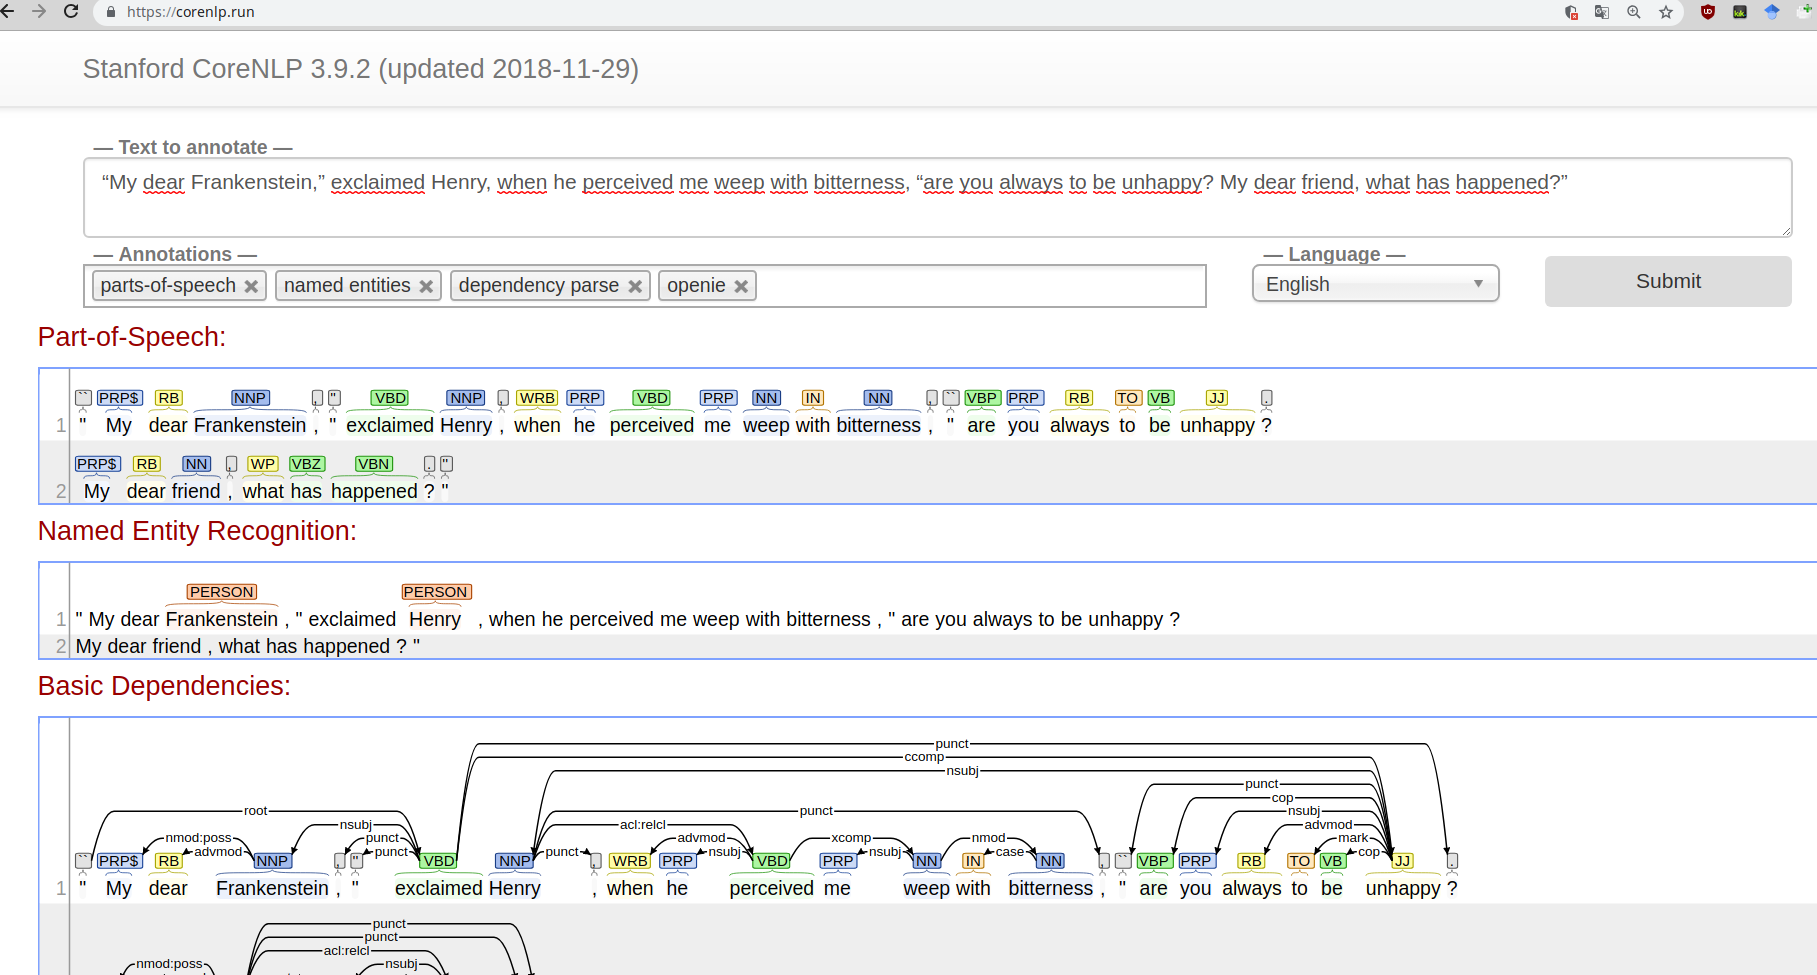
\includegraphics[width=0.9\textwidth]{img/frankenstein-corenlp.png}


\end{frame}
%------------------------------------------------------------------------------

\begin{frame}[allowframebreaks]{Datenvisualisierungen aus quantitativer Textanalyse}
Beispiel Rolling Window; 
\href{http://www.thomaswilhelm.eu/shakespeare/output/hamlet.html}{To See Or Not to See: Shakespeare-Visualisierung} (annotationsbasiert, d.h. XML-Daten)

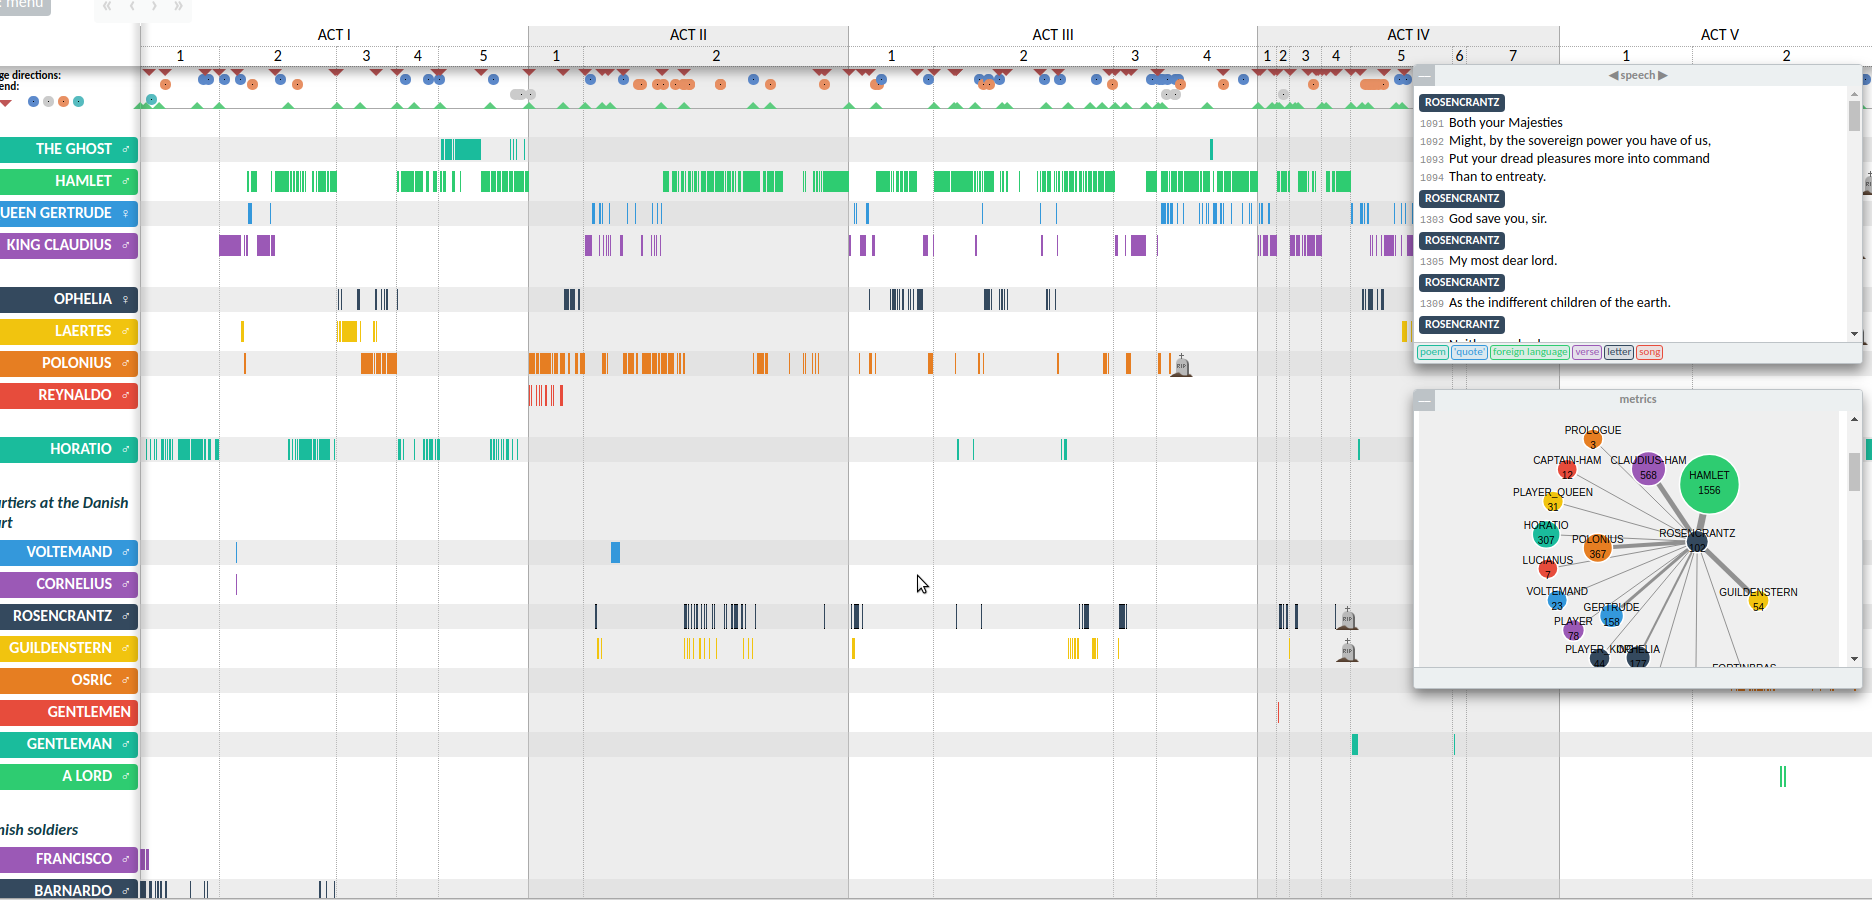
\includegraphics[width=\textwidth]{img/toSeeOrNotToSee.png}

\framebreak

\href{https://www.jasondavies.com/wordtree/}{WordTree}

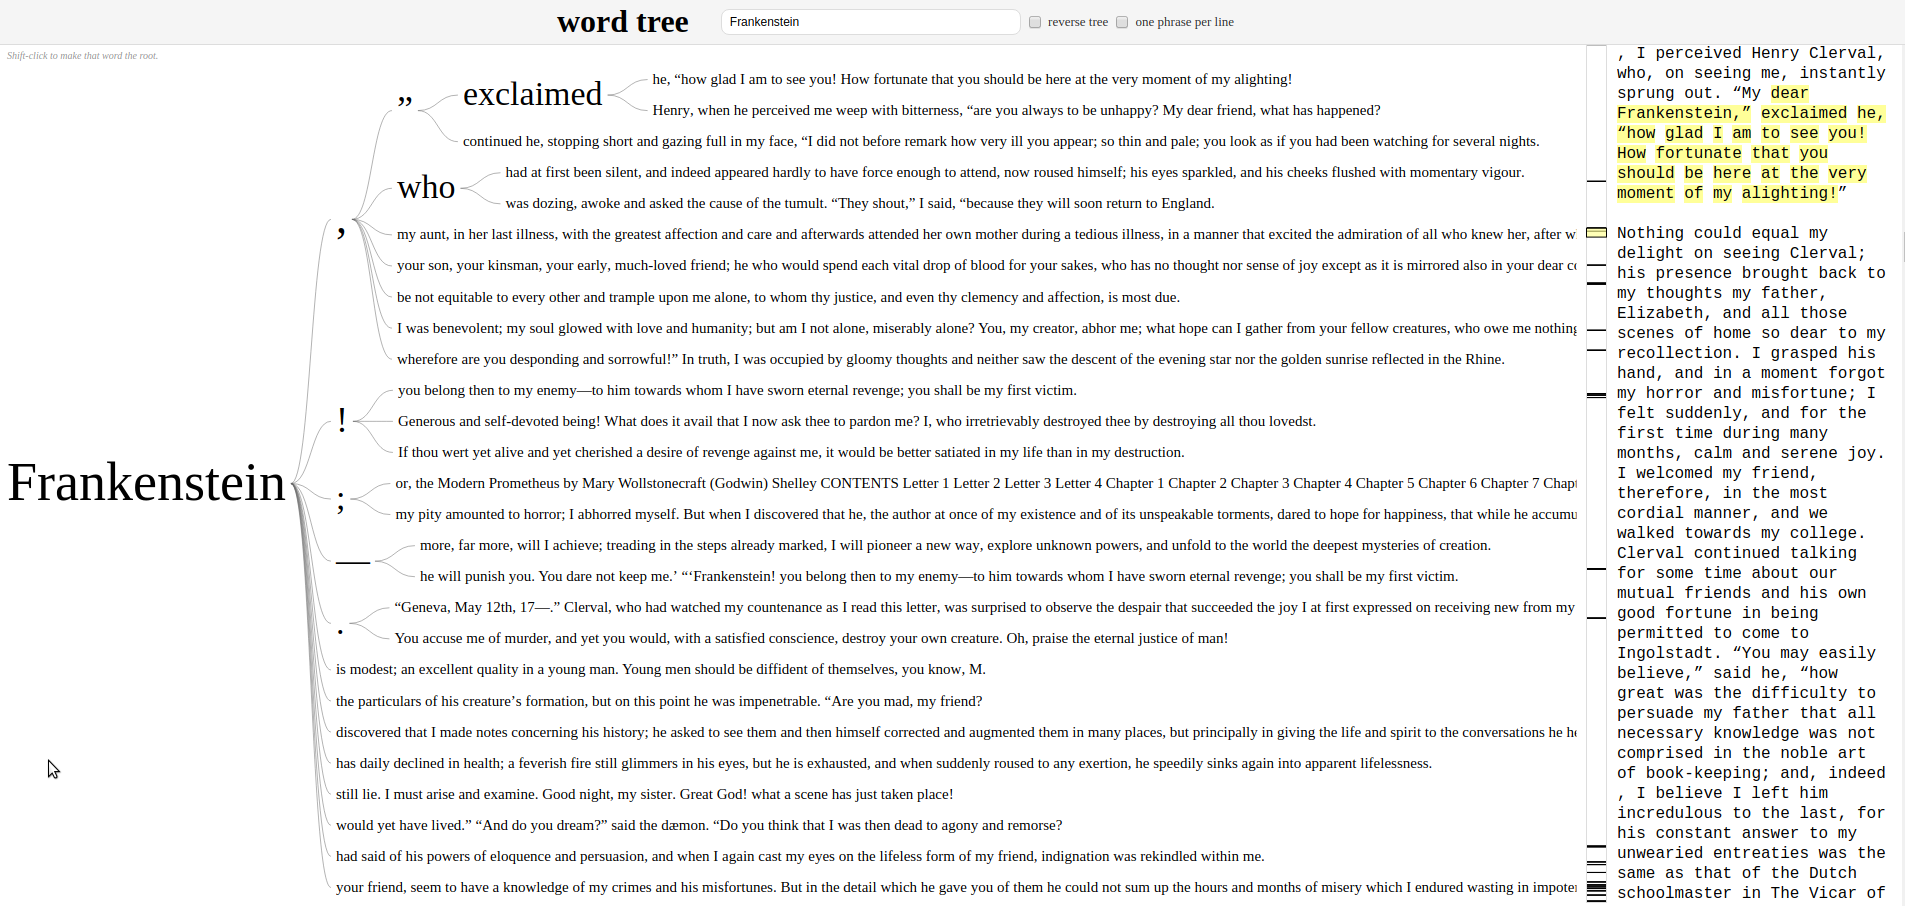
\includegraphics[width=\textwidth]{img/wordTree.png}

\framebreak

\href{https://blogs.reed.edu/ed-tech/2017/03/text-analysis-using-voyant-tools/}{Blogpost zu Voyant} \sep \href{https://voyant-tools.org/}{Voyant Tools}

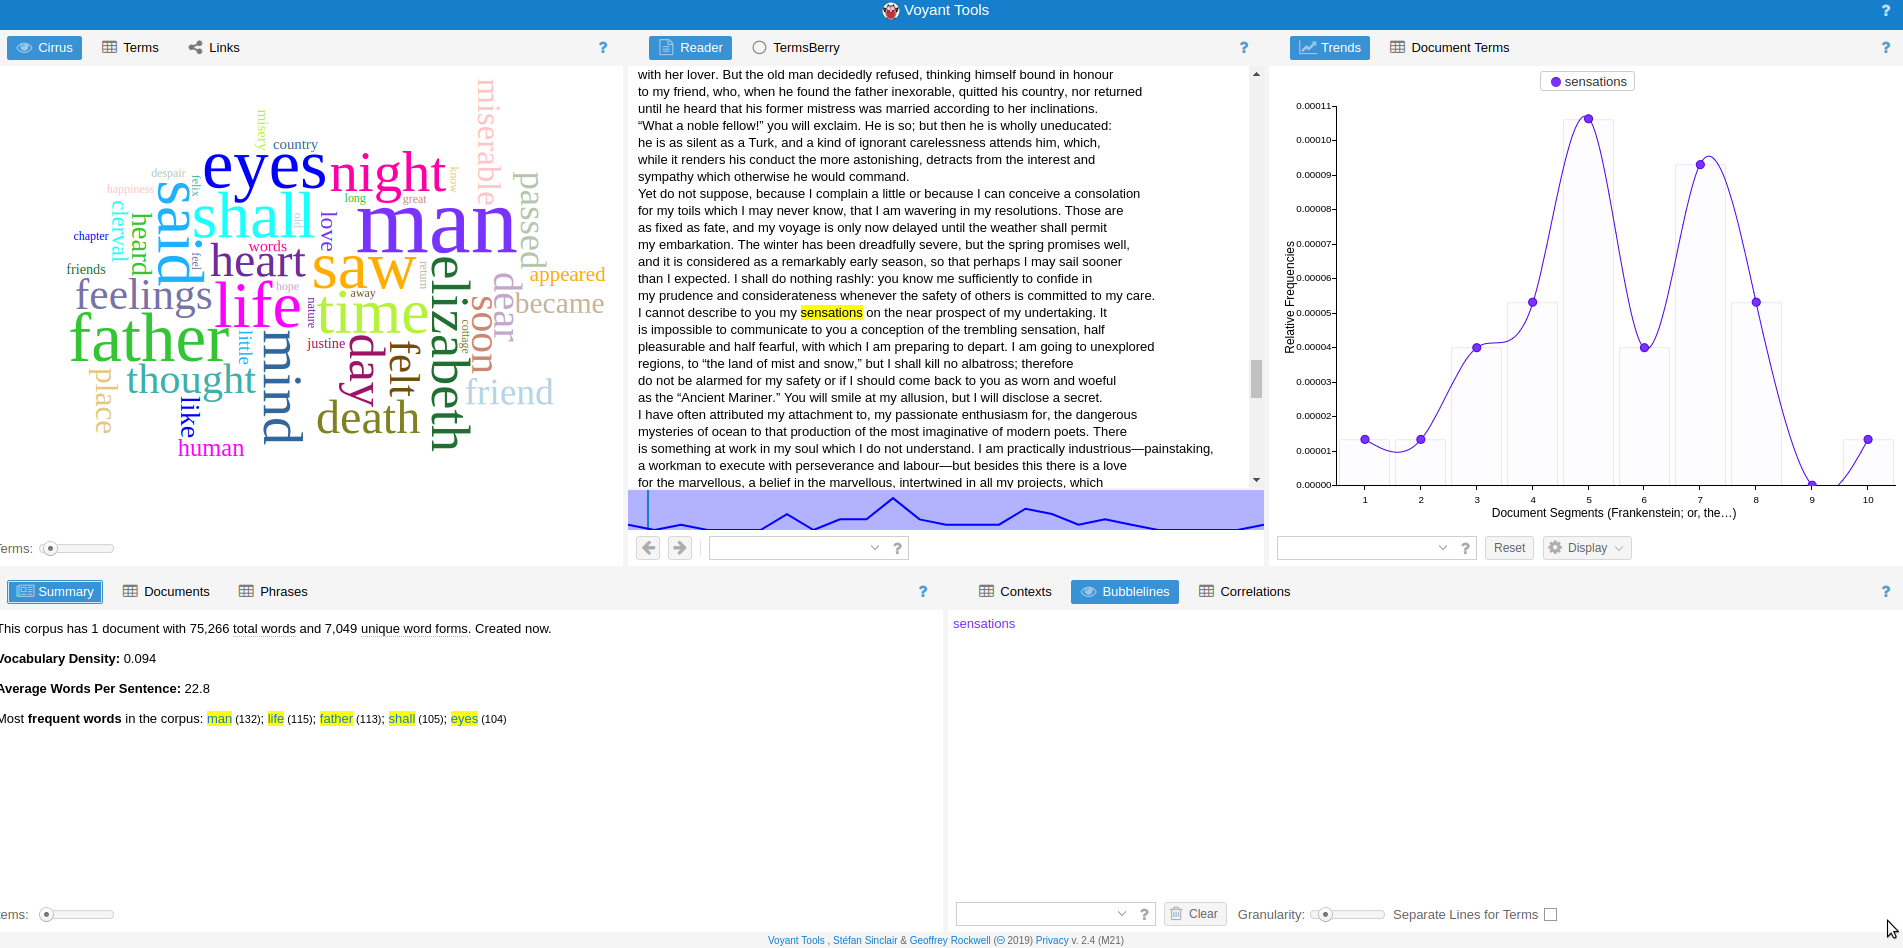
\includegraphics[width=\textwidth]{img/voyant.png}
\end{frame}
%------------------------------------------------------------------------------

\begin{frame}{Buch-Tipps zum Einstieg}

\href{https://www.springer.com/de/book/9783476026224}{
\includegraphics[width=0.45\textwidth]{img/dh-einf.png}}
\hspace{2em}
\href{https://www.nltk.org/book/}{
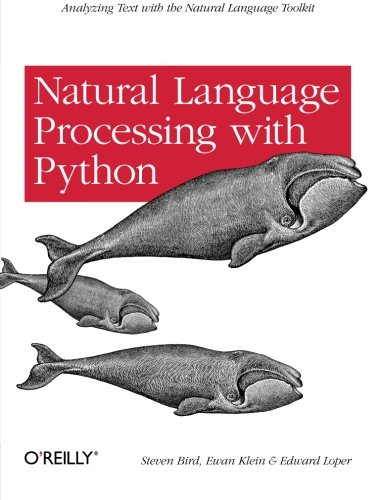
\includegraphics[width=0.45\textwidth]{img/nltk-buch-python.jpg}
}
\end{frame}
%------------------------------------------------------------------------------


%------------------------------------------------------------------------------
\section{Ausblick}
\begin{frame}{Ausblick}
\metroset{block=fill}
    \begin{exampleblock}{Verbindungen zu anderen LVen}
    Viele Inhalte dieser LV werden in anderen LVen noch vertieft.
        \begin{description}\footnotesize
            \item[X-Technologien (1+2)] XML, XPath, XSLT, XQuery, XML-Datenbanken, Textmodellierung
            \item[Einführung in die Programmierung (1+2)] Datenstrukturen und Datentypen
            \item[Webentwicklung] HTML, CSS, JavaScript
            \item[Informationsmodellierung 2] ER, UML; Tabellen, Graphen, Bäume; Fokus auf Graphen/RDF; Abfragen in SQL und SPARQL
            \item[Textmining / Data Science] Vertiefung der hier angeschnittenen Aspekte
            \item[Langzeitarchivierung/Datenmanagement] Umgang mit den Daten
            \item[Grundfragen-Seminar] Was sind DH? Aktuelle Diskurse; Korpus- \& Datenkritik. 
        \end{description}
    \end{exampleblock}
\end{frame}
%------------------------------------------------------------------------------

\begin{frame}[standout]
    Vielen Dank für die gute Zusammenarbeit! \\ 
    \alert{Bitte evaluieren nicht vergessen.}
\end{frame}
